\documentclass[english,,man,floatsintext]{apa6}
\usepackage{lmodern}
\usepackage{amssymb,amsmath}
\usepackage{ifxetex,ifluatex}
\usepackage{fixltx2e} % provides \textsubscript
\ifnum 0\ifxetex 1\fi\ifluatex 1\fi=0 % if pdftex
  \usepackage[T1]{fontenc}
  \usepackage[utf8]{inputenc}
\else % if luatex or xelatex
  \ifxetex
    \usepackage{mathspec}
  \else
    \usepackage{fontspec}
  \fi
  \defaultfontfeatures{Ligatures=TeX,Scale=MatchLowercase}
\fi
% use upquote if available, for straight quotes in verbatim environments
\IfFileExists{upquote.sty}{\usepackage{upquote}}{}
% use microtype if available
\IfFileExists{microtype.sty}{%
\usepackage{microtype}
\UseMicrotypeSet[protrusion]{basicmath} % disable protrusion for tt fonts
}{}
\usepackage{hyperref}
\hypersetup{unicode=true,
            pdftitle={Non-word repetition among the Tsimane': A small-scale study},
            pdfauthor={Alejandrina Cristia, Steven Levinson, \& Marisa Casillas},
            pdfkeywords={phonology, non-word repetition},
            pdfborder={0 0 0},
            breaklinks=true}
\urlstyle{same}  % don't use monospace font for urls
\ifnum 0\ifxetex 1\fi\ifluatex 1\fi=0 % if pdftex
  \usepackage[shorthands=off,main=english]{babel}
\else
  \usepackage{polyglossia}
  \setmainlanguage[]{english}
\fi
\usepackage{graphicx,grffile}
\makeatletter
\def\maxwidth{\ifdim\Gin@nat@width>\linewidth\linewidth\else\Gin@nat@width\fi}
\def\maxheight{\ifdim\Gin@nat@height>\textheight\textheight\else\Gin@nat@height\fi}
\makeatother
% Scale images if necessary, so that they will not overflow the page
% margins by default, and it is still possible to overwrite the defaults
% using explicit options in \includegraphics[width, height, ...]{}
\setkeys{Gin}{width=\maxwidth,height=\maxheight,keepaspectratio}
\IfFileExists{parskip.sty}{%
\usepackage{parskip}
}{% else
\setlength{\parindent}{0pt}
\setlength{\parskip}{6pt plus 2pt minus 1pt}
}
\setlength{\emergencystretch}{3em}  % prevent overfull lines
\providecommand{\tightlist}{%
  \setlength{\itemsep}{0pt}\setlength{\parskip}{0pt}}
\setcounter{secnumdepth}{0}
% Redefines (sub)paragraphs to behave more like sections
\ifx\paragraph\undefined\else
\let\oldparagraph\paragraph
\renewcommand{\paragraph}[1]{\oldparagraph{#1}\mbox{}}
\fi
\ifx\subparagraph\undefined\else
\let\oldsubparagraph\subparagraph
\renewcommand{\subparagraph}[1]{\oldsubparagraph{#1}\mbox{}}
\fi

%%% Use protect on footnotes to avoid problems with footnotes in titles
\let\rmarkdownfootnote\footnote%
\def\footnote{\protect\rmarkdownfootnote}


  \title{Non-word repetition among the Tsimane': A small-scale study}
    \author{Alejandrina Cristia\textsuperscript{1}, Steven Levinson\textsuperscript{2}, \& Marisa Casillas\textsuperscript{2}}
    \date{}
  
\shorttitle{NWR among the Tsimane'}
\affiliation{
\vspace{0.5cm}
\textsuperscript{1} LSCP, Département d’études cognitives, ENS, EHESS, CNRS, Université PSL\\\textsuperscript{2} MPI}
\keywords{phonology, non-word repetition\newline\indent Word count: xxx}
\usepackage{csquotes}
\usepackage{upgreek}
\captionsetup{font=singlespacing,justification=justified}

\usepackage{longtable}
\usepackage{lscape}
\usepackage{multirow}
\usepackage{tabularx}
\usepackage[flushleft]{threeparttable}
\usepackage{threeparttablex}

\newenvironment{lltable}{\begin{landscape}\begin{center}\begin{ThreePartTable}}{\end{ThreePartTable}\end{center}\end{landscape}}

\makeatletter
\newcommand\LastLTentrywidth{1em}
\newlength\longtablewidth
\setlength{\longtablewidth}{1in}
\newcommand{\getlongtablewidth}{\begingroup \ifcsname LT@\roman{LT@tables}\endcsname \global\longtablewidth=0pt \renewcommand{\LT@entry}[2]{\global\advance\longtablewidth by ##2\relax\gdef\LastLTentrywidth{##2}}\@nameuse{LT@\roman{LT@tables}} \fi \endgroup}

\authornote{

Correspondence concerning this article should be addressed to Alejandrina Cristia, 29, rue d'Ulm, 75005, Paris, France. E-mail: \href{mailto:alecristia@gmail.com}{\nolinkurl{alecristia@gmail.com}}}

\abstract{
ADD


}

\begin{document}
\maketitle

\hypertarget{introduction}{%
\subsection{Introduction}\label{introduction}}

\begin{itemize}
\tightlist
\item
  many studies on phonological development in childhood
\item
  they show phonology continues developing as children learn more words and gain mastery of phonetic targets
\item
  one key task in this research in NWR
\item
  used for theory (eg what are the links between phonology, working memory, and lexicon?), and for applications (nwr as a diagnostic)
\item
  it has been used acros a wide array of languages, particularly in Europe
\item
  however, less is known about NWR development in non-Indo European languages
\item
  this study: NWR in a Yêly Dnyé, an isolate spoken in Rossel Island, PNG, with an unusually dense phonological inventory
\end{itemize}

In this study, we use nonword repetition (NWR), a technique that has been widely adopted to study the development of perception-production across multiple languages (CITE), particularly in Europe (CITE). In NWR studies, participants are presented auditorily with an item that is phonologically legal but lexically meaningless in the language children are learning. The child should immediately try to say it back without changing anything. Accuracy is thought to reflect long-term phonological knowledge (which allows the child to perceive the item accurately even though it is not a real word they have encountered before) as well as online working memory (to encode the item in the interval between hearing it and saying it back). In our implementation of NWR, we additionally made sure that some of the items contained typologically rare and/or challenging sounds, to additionally capture children's auditory-articulatory accuracy.

Little is known about language development in children growing up in Rossel Island, a community of primarily subsistence farmers who tend to reside in clise-knitted villages where child care is distributed across many individuals, and who typically speak Yélî Dnyé, a phonologically and lexically complex language.

\hypertarget{intro-to-the-language}{%
\subsubsection{Intro to the language}\label{intro-to-the-language}}

\begin{itemize}
\tightlist
\item
  complexity in the vowel system
\item
  complexity in the consonant system
\item
  word shapes
\item
  typical word length
\item
  although not the focus of this paper, high use of suppletion in verbal paradigms, other features of language, see Levinson XXX for details
\end{itemize}

\hypertarget{intro-to-the-people}{%
\subsubsection{Intro to the people}\label{intro-to-the-people}}

\begin{itemize}
\tightlist
\item
  usually monolingual at home
\item
  schooling in English but it starts at age XX, so not relevant here
\item
  however, some use of English due to immigrants \& children of immigrants
\item
  children spend a lot of time with other children
\item
  most parents are subsistence farmers
\item
  parental education generally varies between XX and YY
\end{itemize}

\hypertarget{brief-review-of-nwr-for-our-purposes}{%
\subsubsection{Brief review of NWR for our purposes}\label{brief-review-of-nwr-for-our-purposes}}

\begin{itemize}
\item
  typical structure of NWR tasks: N of items
\item
  complexity varies widely across tasks, sometimes within tasks on purpose
\item
  some authors modulate structural complexity (nb syll, syllable structure), others familiarity via phonotactic probability
\item
  calculation of frequency in Yêli is challenging bc low resource language
\item
  so we only manipulated structural complexity, not probability
\item
  previous work seems to avoid difficult sounds
\item
  but we felt this was important to represent the language, so we also varied this factor
\item
  previous work shows even 2yo can do the task
\item
  but there are striking changes with age
\item
  inconsistent results RE effects of SES (including parental education) \& child sex
\item
  brief summary of inconsistent results SES
\item
  idem for sex
\end{itemize}

\hypertarget{research-questions-and-predictions}{%
\subsubsection{Research questions and predictions}\label{research-questions-and-predictions}}

\begin{itemize}
\tightlist
\item
  What is the accuracy (whole word, phoneme based, distance) overall?
\item
  How does this change as a function of item complexity (nb syll, syll complexity, sound complexity)?
\item
  How frequent are errors that result in real words? Is that a function of item complexity?
\item
  Is individual variation explainable by child age, sex, parental education?
\end{itemize}

Based on previous work, we made the following predictions:

\begin{enumerate}
\def\labelenumi{\arabic{enumi}.}
\tightlist
\item
  Children are more accurate for mono-syllables than longer items
\item
  Similarly, we do not know of NWR research that manipulates the difficulty of the sounds that are included in the items, but word naming and other research suggests that children are more accurate when producing easy and/or typologically common sounds than difficult and/or typologically rare sounds
\item
  Children's accuracy increases with child age
\item
  Non-monolingual Yélî children are less accurate than monolingual ones when tested on the dominant language (we did not test any non-dominant language)
\item
  Previous NWR evidence on this is mixed, but general findings on language development suggest that children whose mothers are more educated are more accurate than children whose mothers are less educated
\item
  To our knowledge, there is no previous NWR work on this, but other research suggests that first-born children should outperfomr later-born children
\end{enumerate}

Although these predictions were made based on previous work, we also thought reasonable that they would not obtain for the Rossel children in particular, as follows:

\begin{enumerate}
\def\labelenumi{\arabic{enumi}.}
\tightlist
\item
  The length distribution in Yélî words is more balanced than that in English, and thus the performance decline for poly- versus mono-syllables may be less pronounced than that for English. \textbf{Check for work on European languages that may have looked into this}
\item
  The Yélî sound inventory is very large and compressed, with many similar sounds that are acoustic and articulatory neighbors. Therefore, this may constitute a pressure for children to have finer aduitory skills (and perhaps more precise articulations) than children speaking languages with a simpler inventory. \textbf{no work looking at consonants \& vowels? no work looking at nasal vowels in particular?}
\item
  We had no reservations that children's accuracy increases with child age for the Yélî community as well.
\item
  Anecdotally Yélî children grow up in close-knitted communities and thus may receive significant portions of their language input from non-kin (or at least from people other than their mothers, who tend to be the non-native speakers). If so, the difference between monolinguals and not monolinguals may be smaller than that found in other work. That said, one recent study shozs that most child-directed input in the first 2 years does come from the mother, so in so far as this input has a crucial formational role, then there may still be a performance gap between these two groups.
\item
  In the Rossel community, formal education plays an extremely minor role in ensuring individual's success, is not a good index of relative socio-economic status, and furthermore there is only a narrow range of variation in maternal educational attainment. This may lead to no or only very small advantages for children whose mothers are more educated, provided that the causal chain between maternal education and child language is via SES more broadly. However, if education directly boosts maternal verbal skills and the incidence of verbal behavior (as suggested by CITE), then we should still see a difference along this factor.
\item
  One main causal path between birth order and language development is via parental input (CITE). Given our arguments above for how mothers may not be as important among Rossel people than in other places, then the performance gap between first borns and later borns may be smaller.
\end{enumerate}

\hypertarget{pre-registration-and-planned-analyses}{%
\subsection{Pre-registration and planned analyses}\label{pre-registration-and-planned-analyses}}

In view of the hypothesis driven nature of this work, we intended to boost the interpretational value of these data by announcing our analysis plans prior to conducting them. There are a few limitations in our approach:

\begin{itemize}
\tightlist
\item
  The sample size is too small to have enough power to detect all of the relationships of interest
\item
  In fact, the sample size is too small to detect some of the known effects (see Table XX \textbf{add table with r/ds from previous work})
\item
  By virtue of this being a language-specific study, it is unclear that our method (including saliently the items we used) is comparable in precision to previous NWR studies
\item
  Analyses were designed and pre-registered by the same person who collected the data, who coded accuracy (albeit with a non-native ear) on the first 11 participants, and who segmented all children's production. Therefore, a key condition of blinding is not met
\end{itemize}

Nonetheless, some form of pre-registration still seemed preferrable over the complete lack of it.

The pre-registration can be found XXX

\hypertarget{stimuli}{%
\subsection{Stimuli}\label{stimuli}}

Many NWR studies are based on a fixed list of 12-16 items that vary in length between 1 and 4 syllables, often additionally varying syllable complexity and/or cluster presence and complexity, always meeting the condition that they do not mean anything in the target language. We kept the same variation in item length and the non-meaningfulness requirement, but we did not vary syllable complexity and clusters because these are vanishingly rare in the language. We also increased the number of items and individual child would be tested on, so that a child would get up to 23 items to repeat, and we created more items and distributed them across children, so as to increase the coverage, and be able to study more items.

A first list of candidate items was generated in 2018 by selecting simple consonants (LIST) and vowels (LIST) that were combined into CV syllables, further sampling the space of 1- to 4-syllable sequences. These candidates were automatically checked against Levinson's 2015 dictionary and removed from consideration if they appeared in the dictionary. They were further presented orally to three local research assistants, who were asked to repeat them and further say whether they were real words. Any item for which two or more of the assistants reported them having a meaning or some form of association were was excluded.

A second list of candidate items was generated in 2019 by selecting complex consonants and systematically crossing them with all the vowels in the Yelî inventory to produce CV monosyllables. As before, items were automatically excluded if they appeared in the dictionary. Additionally, since hearing vowel length in monosyllables in isolation is challenging, any item that had a short/long real word neighbor was filtered out. Since the phonology and phonetics of Yélî is still in the process of being described (CITE), there could have been undocumented constraints that rendered items illegal. Therefore, we made sure that the precise consonant-vowel sequence occurred in some real word in the dictionary (i.e., that there was a longer word included the monosyllable as a subsequence). These candidates were presented to one informant, for a final check that they did not mean anything. Together with the 2018 selection, they were recorded using a headset XXX and an olympus XXX from the written form presented together with the same item orally. The complete recorded list was finally presented to two more informants, who could repeat all the items and who confirmed there were no real words.

The final list is XX.

A Praat script was written to randomize this list 20 times, and split it into two sublists, to generate 40 different elicitation sets. The split had the following constraint:

\begin{itemize}
\tightlist
\item
  the same 3 items were selected as practice items and used in all 40 elicitation sets
\item
  splits were done within each length group from the 2018 items (i.e., separately for 1, 2, 3, and 4-syllable items); and among onset groups for the difficult monosyllables generated in 2019 (i.e., all the monosyllables starting with tp were split into 2 sublists). Since some of these groups had an odd number of items, one of the sublists was slightly longer than the other (20 versus 23).
\item
  once the sublist split had been done, items were randomized such that all children heard first the 3 practice items in a fixed order (1, 2, and 4 syllables), a randomized version of their sublist selection of difficult onset items, and randomized versions of their 2\_syllables, then 3-syllables, and finally 4-syllable items.
\end{itemize}

The 40 elicitation sets are available online from XXX.

\hypertarget{procedure}{%
\subsection{Procedure}\label{procedure}}

We tried to balance three desiderata: That children would not be unduly exposed to the items before they themselves had to repeat them; that children would feel comfortable doing this task with us; and that the community would feel safe with us doing this task with their children. Moreover, there were also some logistic constraints in terms of the space availability. As a result, the places where elicitation took place varied across the hamlets.

Indeed, we visited four different hamlets once, and attempted to test all eligible childr en present at that time, to prevent the items \enquote{spreading} through hearsay. In the first village, we tested children in five different places, with some children being tested inside their house and others tested on the veranda of a house even if it was not their own. The complete list of places and the ways in which they met the desiderata mentioned above can be found in supplementary materials, under comments for each child (direct link xXX).

The child was donned a headset (xx for most of the children, xx for the rest). For most children, the headset could not stay comfortably on the child's head, and thus it was placed on the child's shoulders, with the microphone carefully placed close to the child's mouth. A local informant sat next to the child, to would provide the instructions and, if needed, coach the child to make sure, using the 3 practice items as well as real words, that they understood that the task was to repeat the items precisely without changing anything. An experimenter delivered the elicitation stimuli to the local informant and the child over headhphones.

The first phase was making sure the child understood the task. This was explained orally and the first training item was presented. Often, children froze and did not say anything. If this happened, then we followed this procedure. First, the informant insisted. If the child still did not say anything, the informant asked the child to repeat a real word, and another, and another. If the child could repeat these correctly, then we provided the recorded training item over headphones again. Most children successfully started repeating the items presented over headphones at this point; a few further needed the local informant to model the behavior (i.e., they would hear the item again, and she would say it; then we would play it again, and ask the child to say it). A small minority still failed to repeat the item after hearing it over headphones. If that occurred, we tried with the second training item, at which point some children got it and could continue. A small minority, however, failed to repeat this one, as well as the third training item, in which case we stopped the test altogether.

NWR studies vary in whether children are provided with several opportunities to hear and say the item. To have a fixed and clear procedure, we decided that items other than the inital three training ones would not be repeated unless the child made an attempt to produce them. If this attempt was judged correct by the local informant, then the experimenter would move on to the next item (whispering this over a headset that was recording a separate track). If the local informant heard a deviation, she indicated to the experimenter that the item needed to be repeated, and up to 5 attempts were allowed.

Whenever siblings from the same family were tested, an attempt was made to test first the older and then the younger child, and always on different elicitaiton sets.

\hypertarget{coding}{%
\subsection{Coding}\label{coding}}

There is an implicit accuracy coding occuring online as a function of whether the local informant asked for the item to be repeated or not. We will call this \enquote{online accuracy}, and it reflects a wholesale impression of whether the item was correctly or incorrectly repeated.

Additionally, the experimenter listened through all recordings and segmented out every child production. For the first 11 participants, she additionally made a judgment of whether the item was correctly or incorrectly repeated, and transcribed what she heard, which provides both an accuracy measure and a qualitative description of what children were actually saying in response to each stimulus. . We call this \enquote{non-native coding,} because this experimenter is not familiar with Yélî and has insufficient training on Yélî sounds, including common allophonic variants, not to mention not having some of the sounds in her native perceptual inventory.

Therefore, we sought additional information by asking a local informant to listen through each child production, paried with the auditory target the child had been provided with, and make a judgment of whether the item was correctly or incorrectly repeated. We additionally asked her to transcribe exactly what the child said, providing some examples of the types of errors children in general make (without making specific reference to Yélî sounds or the items in the elicitation sets). This \enquote{native coding} provides both accuracy and qualtiative desciptions of what the child said that are likely more reliable than those of the non-native coder.

\hypertarget{analyses}{%
\subsection{Analyses}\label{analyses}}

For NWR accuracy, we considered only the child's first attempt, which was scored as correct or incorrect online, by a non-native coder (ofr the first 11 kids), and a native coder.

Some NWR studies employ phoneme accuracy (rather than whole word accuracy). We used exclusively the native coding for these, and we calculated accuracy as the number of phonemes that could be aligned across the target and attempt, divided by the number of phonemes of whichever item was longer (the target or the attempt).

Finally, for describing children's patterns of errors, all repetitions of a given target were taken into account, again using only the native coder's transcriptions.

\hypertarget{participants}{%
\subsection{Participants}\label{participants}}

Total N of kids, N of families, N of villages. Some children could not be included for the following reasons: refused participation (N=2), failed to repeat items presented over headphones even after coaching (N=3), spoke too softly to allow offline coding (N=8). In addition, one teenager was tested to put children at ease; their data is not included in analyses below. The remaining XX exhibited the following demographic characteristics

INSERT TABLE WITH THE KEY VARS MENTIONED ABOVE:

\begin{itemize}
\tightlist
\item
  child age
\item
  monoling
\item
  mat ed
\item
  birth order
\end{itemize}

\begin{verbatim}
##  [1] "X.3"         "ID"          "included"    "Age"         "DOB.ISO"    
##  [6] "DOB"         "Sex"         "birthOrder"  "familyID"    "monolingual"
## [11] "matEd"       "Cond"        "Date"        "Time"        "File"       
## [16] "fastcode"    "fullcode"    "Notes"       "Where"       "Village"    
## [21] "X"           "X.1"         "X.2"         "dob"         "test"       
## [26] "age.exact"
\end{verbatim}

\begin{verbatim}
##     ID score.online
## 1  c70    0.7307692
## 2  c71    0.5384615
## 3  c72    0.6086957
## 4  c73    0.8461538
## 5  c74    0.9090909
## 6  c76    0.7307692
## 7  c77    0.9565217
## 8  c78    0.8461538
## 9  c79    0.7692308
## 10 c80    0.8260870
## 11 c81    0.5652174
## 12 c82    0.5000000
\end{verbatim}

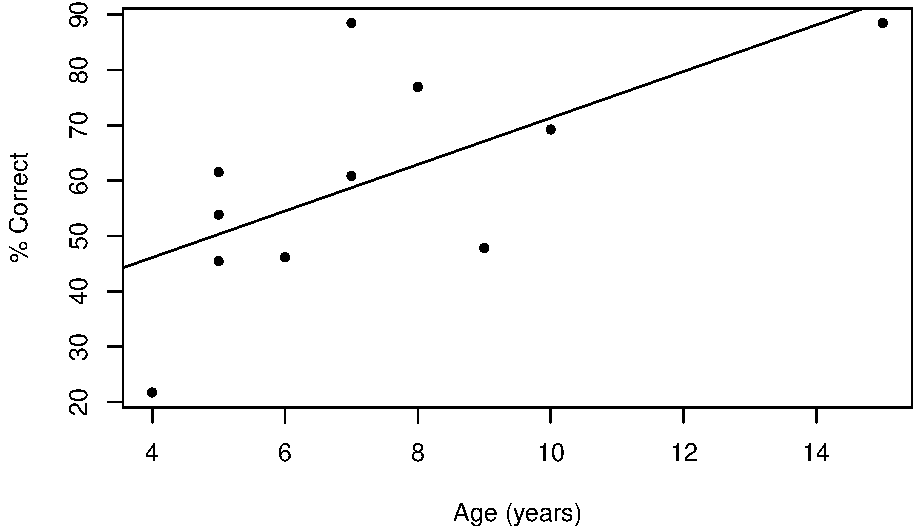
\includegraphics{manuscript_files/figure-latex/cars-1.pdf} 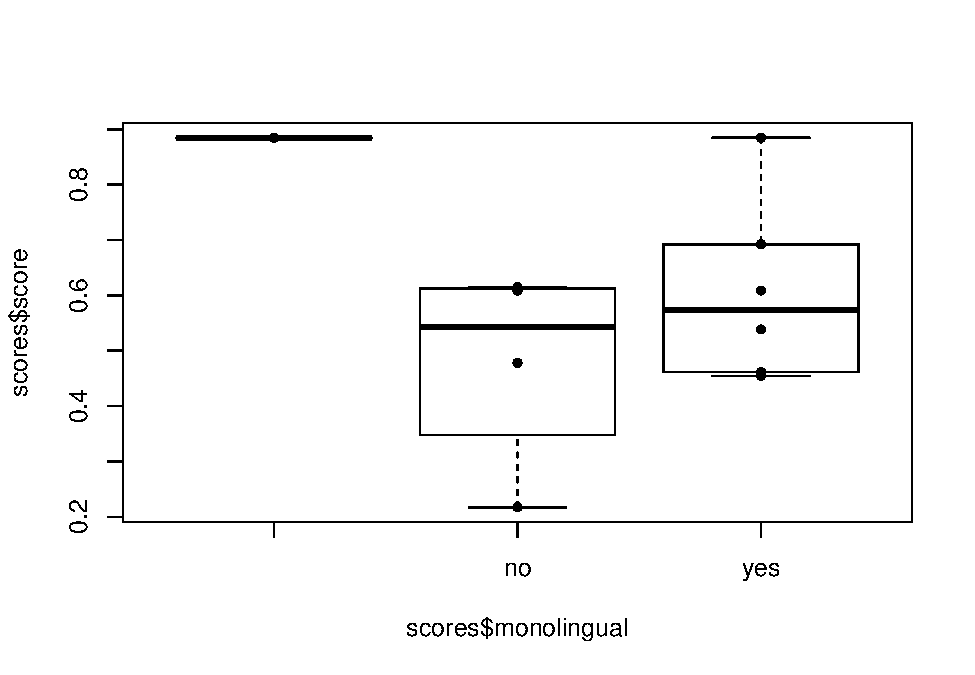
\includegraphics{manuscript_files/figure-latex/cars-2.pdf} 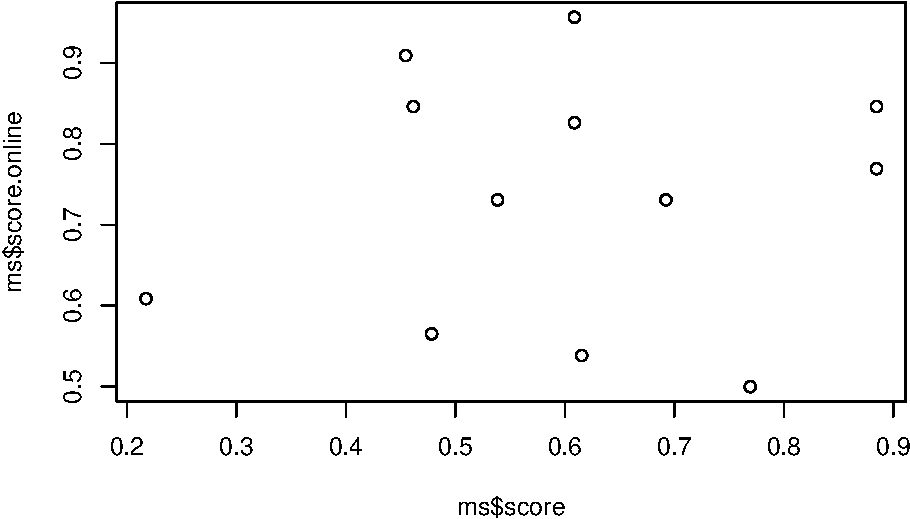
\includegraphics{manuscript_files/figure-latex/cars-3.pdf}

\hypertarget{discussion}{%
\subsection{Discussion}\label{discussion}}

\newpage

\hypertarget{acknowledgments}{%
\subsection{Acknowledgments}\label{acknowledgments}}

We are grateful to informants and individuals who participated in the study. AC acknowledges financial and institutional support from Agence Nationale de la Recherche (ANR-17-CE28-0007 LangAge, ANR-16-DATA-0004 ACLEW, ANR-14-CE30-0003 MechELex, ANR-17-EURE-0017) and the J. S. McDonnell Foundation Understanding Human Cognition Scholar Award.

\hypertarget{references}{%
\section{References}\label{references}}

\setlength{\parindent}{-0.5in}
\setlength{\leftskip}{0.5in}


\end{document}
